\subsection{Installer l'échantillon sur le microscope}
\begin{enumerate}
    \item Retirer la cuvette de liquide fluorescent. L'essuyer avec soin.
    \item \label{observations} Répéter les étapes \ref{ref1} à \ref{ref2} de la section~\ref{ssec:aligner_la_cam} avec la cuvette contenant l'échantillon à imager.
    \\ Note: Avant d'installer l'échantillon sur le microscope, bien étudier sa forme et l'orientation à laquelle on le place par rapport au montage. Ces observations seront très utiles lorsqu'il sera temps de \textit{Saisir les paramètres de scan 3D}.
    
    \item Changer le filtre (voir figure~\ref{fig:filtres}) si nécessaire.
    \item Mettre la couverture noire comme sur la figure~\ref{fig:couverture}. Attention: La couverture ne doit pas se retrouver sur le parcours du laser!
        \begin{figure}[H]
        \centering
        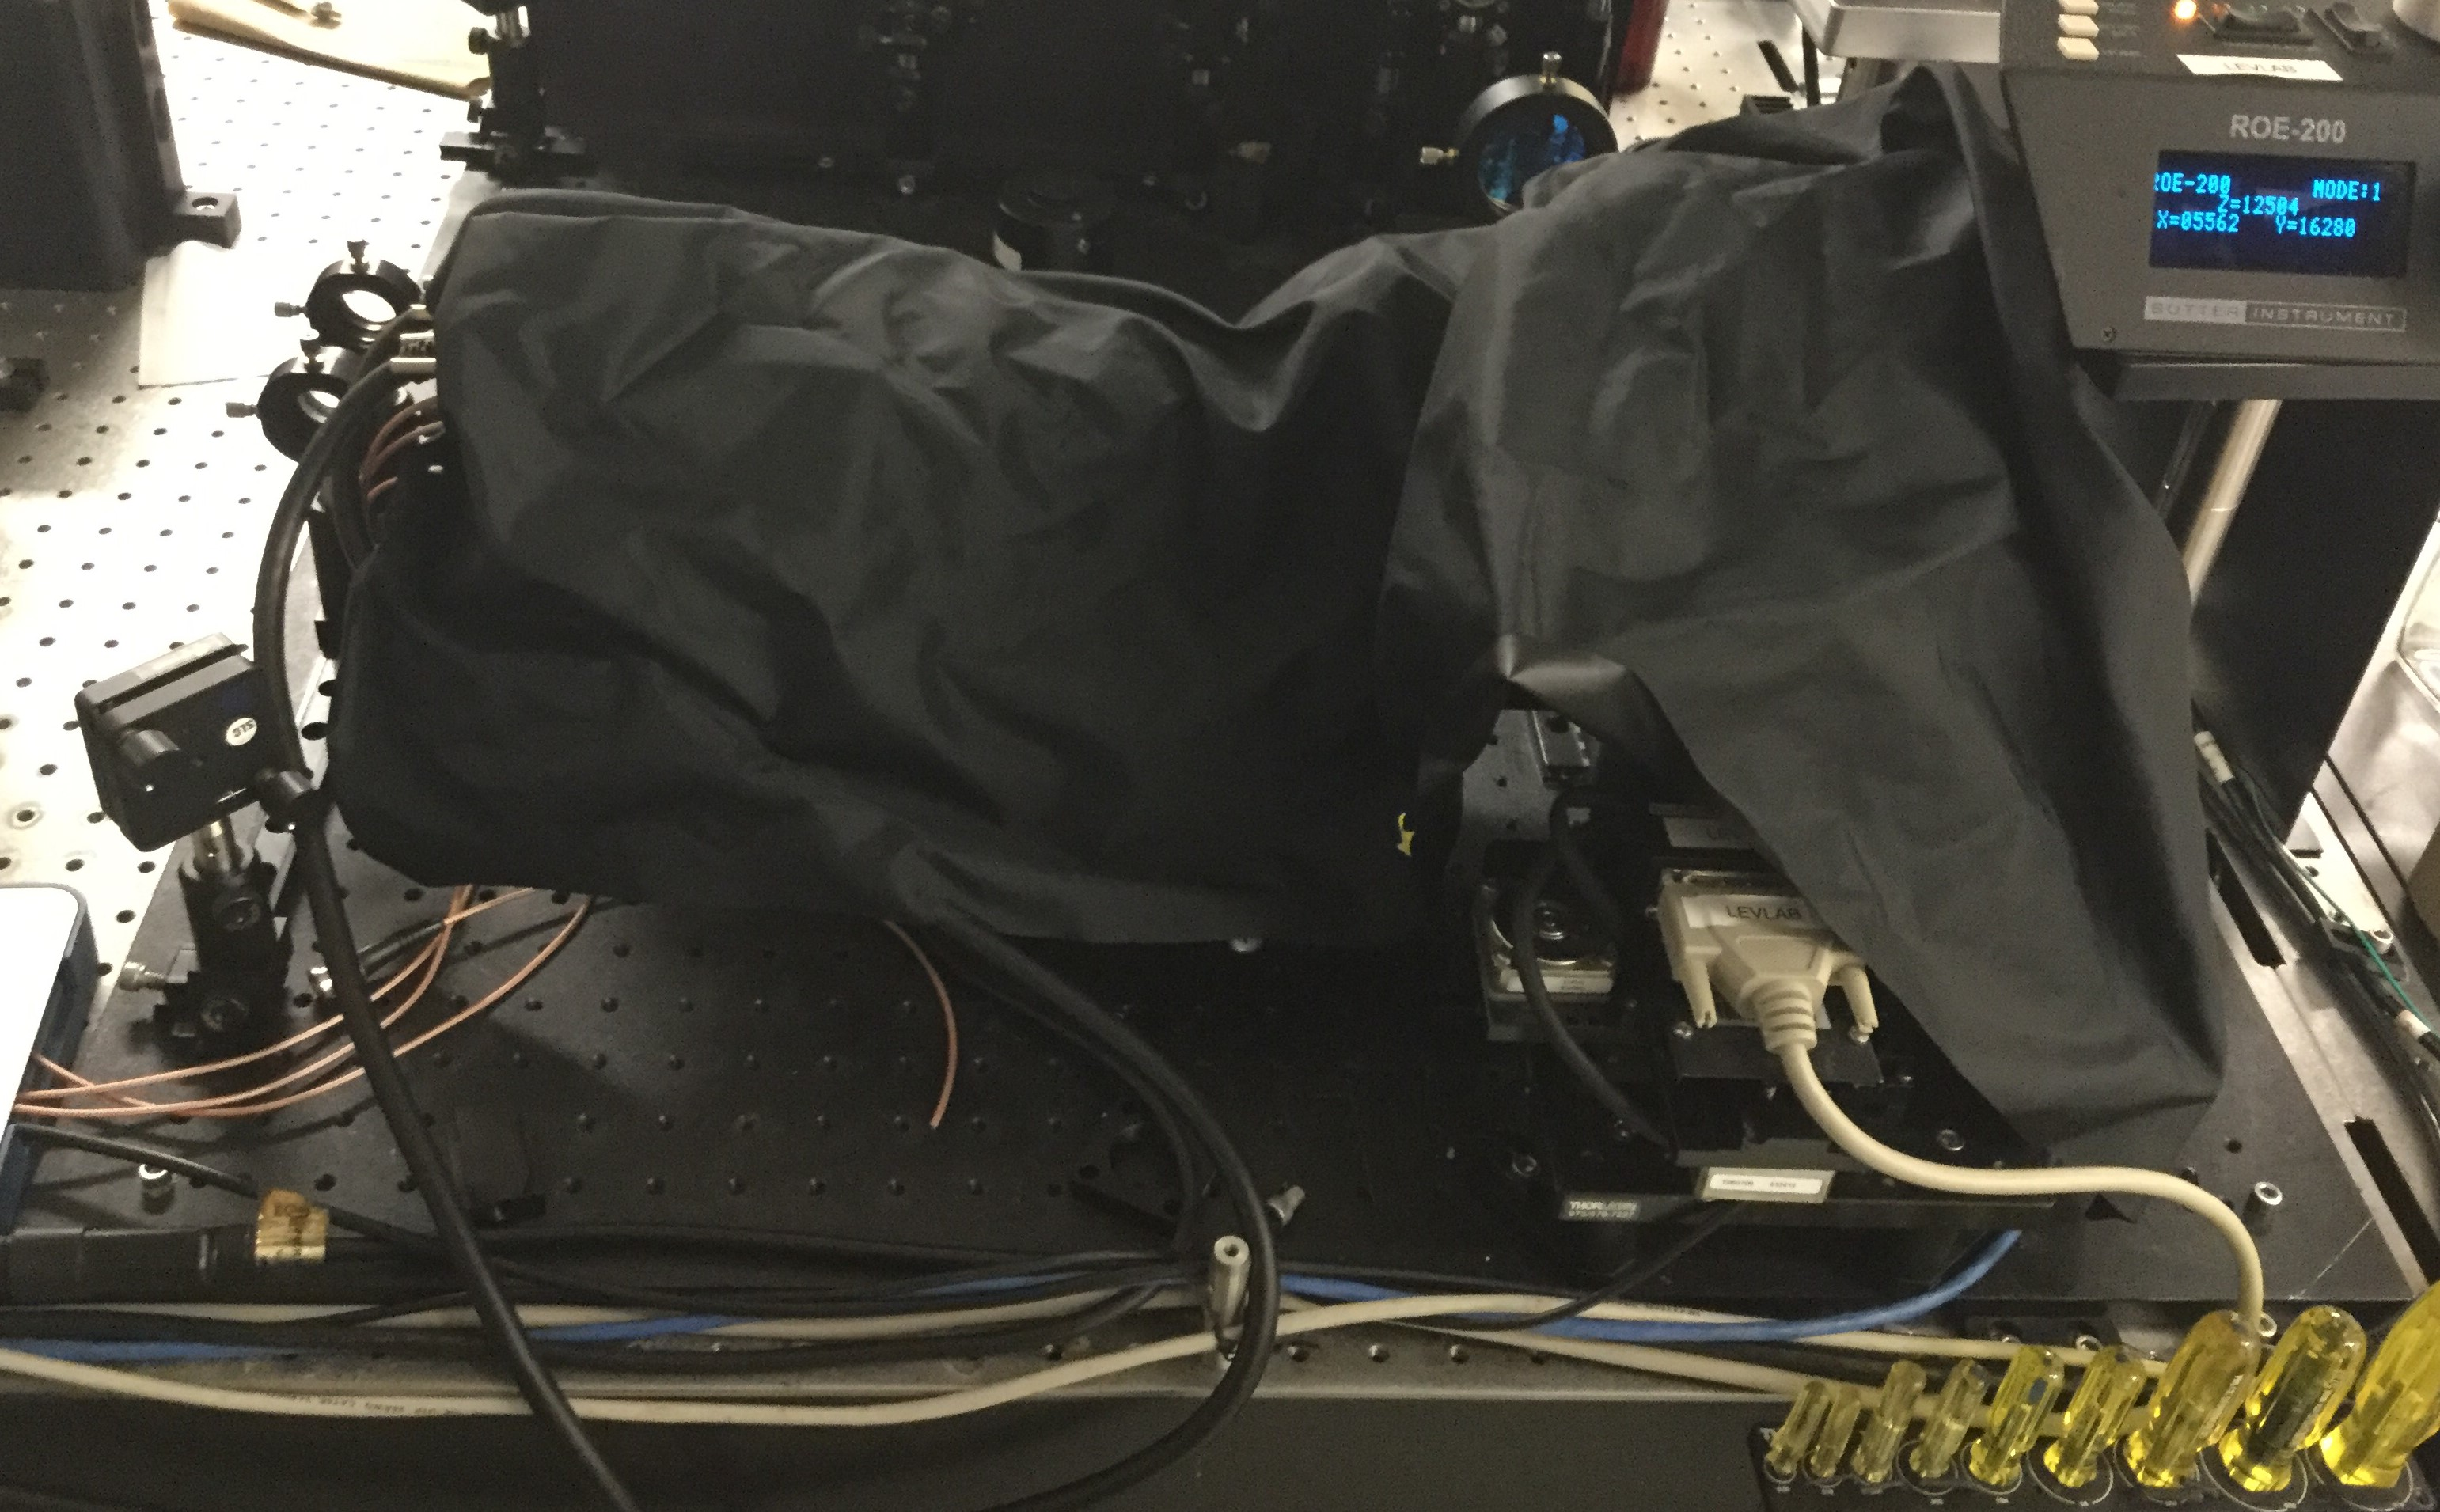
\includegraphics[width=8cm]{couverture.jpg}
        \caption{Couverture sur le montage}
        \label{fig:couverture}
        \end{figure}
    
    \item Cliquer sur \textit{Scan. and Trig.} (6e bouton).
    \item Cliquer sur le menu déroulant indiqué à la figure~\ref{fig:tiret}. Sélectionner l'option '-'. Cliquer sur X pour fermer la fenêtre.
    \item Au besoin, ajuster le contraste ou le temps d'exposition (interface d'accueil (voir figure~\ref{fig:accueil}~-->~\textit{Camera}~->~\textit{Exposure}).
   \item Ajuster la position en profondeur de la caméra à l'aide la \textit{vis C} (voir figure~\ref{fig:vis}).
    \\ But: Avoir la ligne de fluorescence au focus, i.e. avoir la ligne la plus nette/fine possible.
    \item Utiliser les outils d'alignement si nécessaire.
    \item Remettre à l'option '$\uparrow\downarrow$'.
\end{enumerate}